\subsection{Gaussian Blur}
\label{sec:results_gaussian}

\subsubsection{Korrektheit}

Abbildung~\ref{fig:gaussian_result} zeigt das Ergebnis der Filterung im
Vergleich zum Originalbild.

\begin{figure}[H]
    \centering
    
\includegraphics[width=0.7\textwidth]{98_assets/maple-leaf-black-5120x2880-cmp-original-gaussian.jpg}
    \caption{Vergleich Original (links) vs.\ Gaussian Blur (rechts,
        $\sigma = 25$, \texttt{BLUR\_RADIUS}$= 12$). Die Parameter wurden
        bewusst extrem gewählt, um den Effekt deutlicher sichtbar zu machen,
        in der Pipeline wird ein deutlich sanfterer Filter verwendet.}
    \label{fig:gaussian_result}
\end{figure}

\subsubsection{Performance}

Das NCU-Profiling der naiven Implementierung zeigt, dass 47\,\% aller
Global Memory Zugriffe uncoalesced sind, was die in
Abschnitt~\ref{sec:shared_memory_gaussian} beschriebene Shared Memory
Optimierung motiviert.

Der gemessene Speedup hängt stark vom \texttt{BLUR\_RADIUS} ab (Abbildung~\ref{fig:gaussian_ncu}).
Bei $r=2$ sinkt die Kernel-Laufzeit trotz nahezu identischem SM Throughput
bereits um 40.7\,\% (1.69$\times$), bei r = 9 verstärkt sich dieser Effekt
auf einen Speedup von 3.0$\times$ bei deutlich gesteigertem SM Throughput,
da hier die 361 Faltungsoperationen pro Pixel den redundanten
DRAM-Traffic zum dominanten Faktor machen.

Die Pinned-Memory-Variante bestätigt, dass Compute Throughput und
Occupancy bei $r=9$ praktisch identisch zur Shared Memory Variante
sind, da der Kernel selbst unverändert bleibt. Der Vorteil zeigt sich
ausschließlich im D$\to$H-Transfer, der bei $r=9$ von 2.04\,ms auf
1.37\,ms sinkt. Die vollständigen Messdaten sind in Anhang~A
(S.~\pageref{app:gaussian_rohdaten}) aufgeführt.

\begin{figure}[H]
    \centering
    \begin{minipage}{0.48\textwidth}
        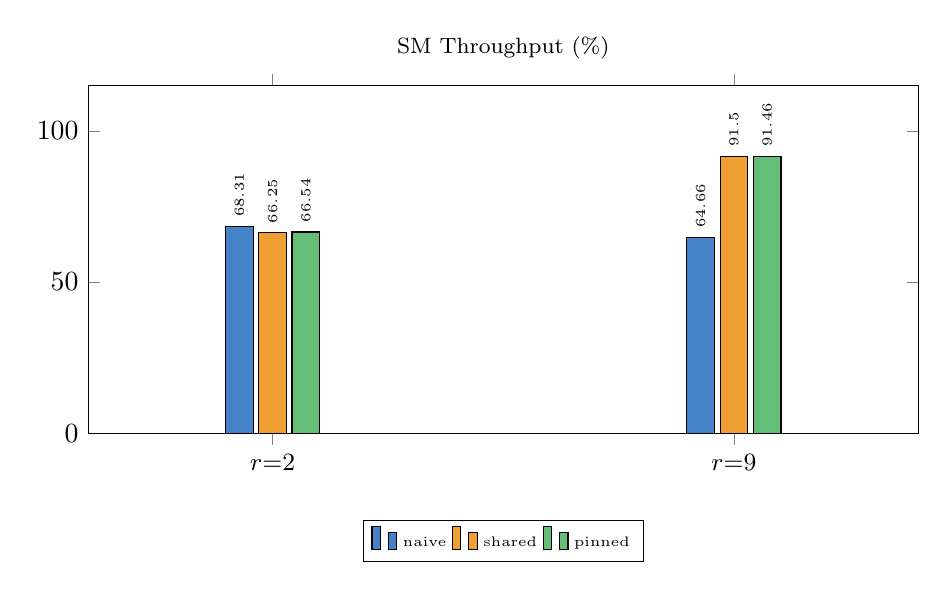
\begin{tikzpicture}
            \begin{axis}[
                ybar,
                bar width=10pt,
                title={SM Throughput (\%)},
            title style={font=\footnotesize},
            xtick={1,2},
            xticklabels={$r{=}2$, $r{=}9$},
            xticklabel style={font=\small},
            width=\textwidth, height=6cm,
            ymin=0, ymax=115,
            enlarge x limits=0.4,
            legend style={at={(0.5,-0.25)}, anchor=north, legend columns=3, font=\tiny},
            nodes near coords,
            nodes near coords style={font=\tiny, rotate=90, anchor=west},
            ]
                \addplot[fill={rgb,255:red,70;green,130;blue,200}]  coordinates {(1,68.31) (2,64.66)};
                \addplot[fill={rgb,255:red,240;green,160;blue,50}]  coordinates {(1,66.25) (2,91.50)};
                \addplot[fill={rgb,255:red,100;green,190;blue,120}] coordinates {(1,66.54) (2,91.46)};
                \legend{naive, shared, pinned}
            \end{axis}
        \end{tikzpicture}
    \end{minipage}
    \hfill
    \begin{minipage}{0.48\textwidth}
        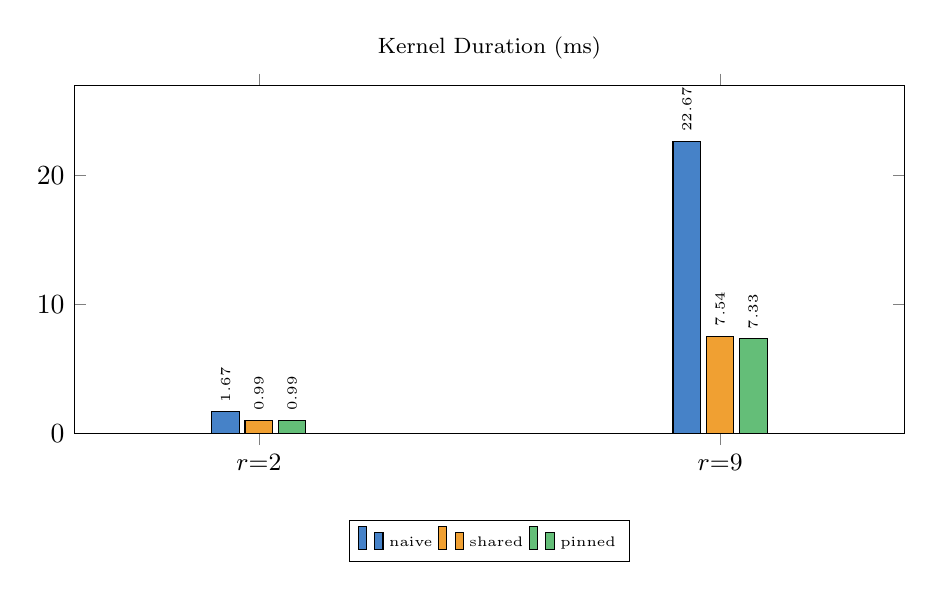
\begin{tikzpicture}
            \begin{axis}[
                ybar,
                bar width=10pt,
                title={Kernel Duration (ms)},
            title style={font=\footnotesize},
            xtick={1,2},
            xticklabels={$r{=}2$, $r{=}9$},
            xticklabel style={font=\small},
            width=\textwidth, height=6cm,
            ymin=0, ymax=27,
            enlarge x limits=0.4,
            legend style={at={(0.5,-0.25)}, anchor=north, legend columns=3, font=\tiny},
            nodes near coords,
            nodes near coords style={font=\tiny, rotate=90, anchor=west},
            ]
                \addplot[fill={rgb,255:red,70;green,130;blue,200}]  coordinates {(1,1.67) (2,22.67)};
                \addplot[fill={rgb,255:red,240;green,160;blue,50}]  coordinates {(1,0.99) (2, 7.54)};
                \addplot[fill={rgb,255:red,100;green,190;blue,120}] coordinates {(1,0.99) (2, 7.33)};
                \legend{naive, shared, pinned}
            \end{axis}
        \end{tikzpicture}
    \end{minipage}
    \caption{NCU-Profiling, Vergleich naive/shared/pinned bei $r{=}2$ und $r{=}9$ (200 Runs Avg).}
    \label{fig:gaussian_ncu}
\end{figure}